\documentclass[a4paper]{article}

\usepackage[utf8]{inputenc}
\usepackage[T1]{fontenc}
\usepackage{textcomp}
\usepackage{listings}
\usepackage{lmodern}
\usepackage{amsfonts}
\usepackage{titling}
\usepackage{lipsum}
\usepackage[left=1in, right=1in, bottom=1in, top=1in]{geometry}
\usepackage{amsthm}
\usepackage{tcolorbox}
\usepackage{hyperref}
\usepackage{xcolor}
\usepackage{graphicx}
\usepackage{makeidx}
\usepackage{tikz}
\usetikzlibrary{calc, arrows, positioning}
\tikzset{
  prefix after node/.style={prefix after command=\pgfextra{#1}},
  /semifill/ang/.initial=45,
  /semifill/upper/.initial=none,
  /semifill/lower/.initial=none,
  semifill/.style={
    circle, draw,
    prefix after node={
      \pgfqkeys{/semifill}{#1}
      \path let \p1 = (\tikzlastnode.north), \p2 = (\tikzlastnode.center),
                \n1 = {\y1-\y2} in [radius=\n1]
            (\tikzlastnode.\pgfkeysvalueof{/semifill/ang})
            edge[
              draw=none,
              fill=\pgfkeysvalueof{/semifill/upper},
              to path={
                arc[start angle=\pgfkeysvalueof{/semifill/ang}, delta angle=180]
                -- cycle}] ()
            (\tikzlastnode.\pgfkeysvalueof{/semifill/ang})
            edge[
              draw=none,
              fill=\pgfkeysvalueof{/semifill/lower},
              to path={
                arc[start angle=\pgfkeysvalueof{/semifill/ang}, delta angle=-180]
                -- cycle}] ();}}}
\usepackage{cases}
\usepackage{apacite}
\usepackage{tkz-berge}
\usepackage{url}
\usepackage{tgtermes}
\usepackage{sectsty}
\usepackage{subcaption}
\usepackage{setspace}
\usepackage{float}
\usepackage{amsmath, amssymb}


% figure support
\usepackage{import}
\usepackage{xifthen}
\pdfminorversion=7
\usepackage{pdfpages}
\usepackage{transparent}
\usepackage{color}
\newcommand{\incfig}[2][1]{%
    \def\svgwidth{#1\columnwidth}
    \import{./figures/}{#2.pdf_tex}
}

%mathstyling
\theoremstyle{plain}
\newtheorem{thm}{Theorem}[section]
\newtheorem{lem}[thm]{Lemma}
\newtheorem{prop}[thm]{Proposition}
\newtheorem*{cor}{Corollary}

\theoremstyle{definition}
\newtheorem{defn}{Definition}[section]
\newtheorem{conj}{Conjecture}[section]
\newtheorem{exmp}{Example}[section]
\newtheorem{axiom}{Axiom}
\theoremstyle{remark}
\newtheorem*{rem}{Remark}
\newtheorem*{note}{Note}

\definecolor{darkgreen}{rgb}{0.0, 0.5, 0.0}

\pdfsuppresswarningpagegroup=1
\lstset{
tabsize = 4, %% set tab space width
showstringspaces = false, %% prevent space marking in strings, string is defined as the text that is generally printed directly to the console
numbers = left, %% display line numbers on the left
commentstyle = \color{darkgreen}, %% set comment color
keywordstyle = \color{blue}, %% set keyword color
stringstyle = \color{red}, %% set string color
rulecolor = \color{black}, %% set frame color to avoid being affected by text color
basicstyle = \small \ttfamily , %% set listing font and size
breaklines = true, %% enable line breaking
numberstyle = \tiny,
  frame=none,
  xleftmargin=2pt,
  stepnumber=1,
  belowcaptionskip=\bigskipamount,
  captionpos=b,
  escapeinside={*'}{'*},
  language=haskell,
  tabsize=2,
  emphstyle={\bf},
  showspaces=false,
  columns=flexible,
  showstringspaces=false,
  morecomment=[l]\%,
}
\begin{document}
	\begin{titlepage}
	\begin{center}
	\large
	University of Warwick \\
	Department of Computer Science \\
	\huge
	\vspace{50mm}
	\rule{\linewidth}{0.5pt} \\
	CS331 \\
	\vspace{5mm}
	\Large
	Neural Computing
	\rule{\linewidth}{0.5pt}
	\vspace{5mm}
	\begin{figure}[H]
	\centering
	
\includegraphics[width=0.4\textwidth]{crest_black.eps}
	\end{figure}
	\vspace{37mm}
	Cem Yilmaz \\
	\today
	\end{center}
	\end{titlepage}
	\newpage
	\section{Question 1}
	\subsection{(a)}
	For the function
	\begin{align*}
		f(x_1,x_2,x_3) = (x_1 \text{NIMPLY}x_2) \text{NIMPLY} x_3
	\end{align*}
	We can construct its truth table as follows:
	\begin{table}[H]
		\centering
		\caption{$f(x_1,x_2,x_3)$ truth table}
		\label{tab:f}
		\begin{tabular}{|c|c|c|c|}
			\hline
		$x_1$ & $x_2$ &$x_3$  & $f(x_1,x_2,x_3)$ \\
		\hline
		F & F & F & F \\
		F & F & T & F \\
		F & T & F & F \\
		F & T & T & F \\
		T & F & F & T \\
		T & F & T & F \\
		T & T & F & F \\
		T & T & T & F \\
		\hline
		\end{tabular}
	\end{table}
\noindent From this table, notice that we only have a single T value, which is true if $x_1$ is true, $x_2$ is false and $x_3$ is false. Therefore, we can deduce that it is always false whenever $x_2$ or $x_3$ are true, as such, we can define them as inhibitory, i.e., when $x_2$ or $x_3$ is $T=1$, the output is always $F=0$. This leaves us a case at which $f$ as a neuron can only fire when $x_2,x_3=0$, which means that now it is only dependent on $x_1$. There are two combinations: $x_1 = 1$ or $x_1=0$. In this  case, we just have to define $\theta = 1$, that is, $z \ge 1$ to ensure that we fire when $x_1$ is $T=1$.	
\begin{figure}[H]
	\centering
	\begin{tikzpicture}
		\node[semifill={lower=black, ang=90}, scale=3] (r) at (0,0) {};
		\node[draw, shape=circle, scale=0.6] (s) at (-0.6,0) {};
		\node[draw, shape=circle, scale=0.6] (ss) at (-0.55,-0.25) {};
		\node[text] at (-0.2,0) {$2$ };
		\node[text] (x1) at (-3, 0) {$x_2$};
		\node[text] (f) at (3,0) {$f$ };
		\node[text] (x2) at (-3,1.5) { $x_1$ };
		\node[text] (x3) at (-3,-1.5) {$x_3$ };
		\path [->] (x1) edge (s);
		\path [->] (x2) edge (r);
		\path [->] (x3) edge (ss);
		\path [->] (r) edge (f);
	\end{tikzpicture}
	\caption{Rojas diagram of $f$}
	\label{fig:rojas}
\end{figure}
\subsection{(b)}
\begin{figure}[H]
	\centering
	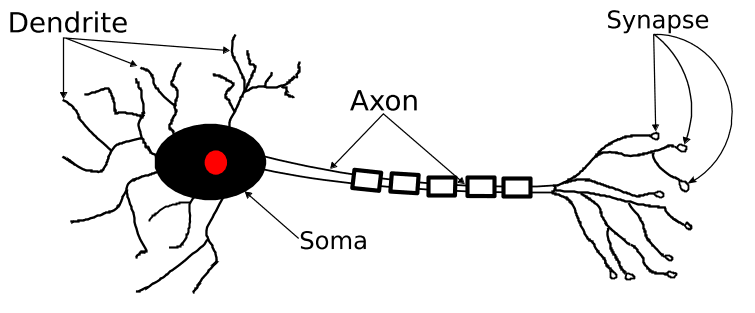
\includegraphics[width=0.8\textwidth]{neuron.png}
	\caption{Biological Neuron}
	\label{fig:neuron-png}
\end{figure}
Two main factors that influence the speed of signal transmission along the axon:
\begin{enumerate}
	\item Myelination - myelin acts as an insulator for the charge, creating saltatory conduction. That is, through the process of polarisation and depolarisation of Na${}^+$ and K${}^+$ ions, it is able to create action potential between each myelin which allows it to skip distances.
	\item Diameter - higher diameter of axon means that there is less resistance during signal transmission as the electrical charge (ions) flow more freely.
\end{enumerate}
\subsection{(c)}
$f$ can be emulated by a single-layer perceptron. Consider a 3D plane with its axis defined as $x_1,x_2,x_3$. We notice that the function forms a discrete $2 \times 2 \times 2$ cube, for which $(1,1,1)$ resides on the corner. We can simply create a slanted flat 2D plane $x+y+z=2.5$ that cuts the corner only as shown in the figure below:
\begin{figure}[H]
	\centering
	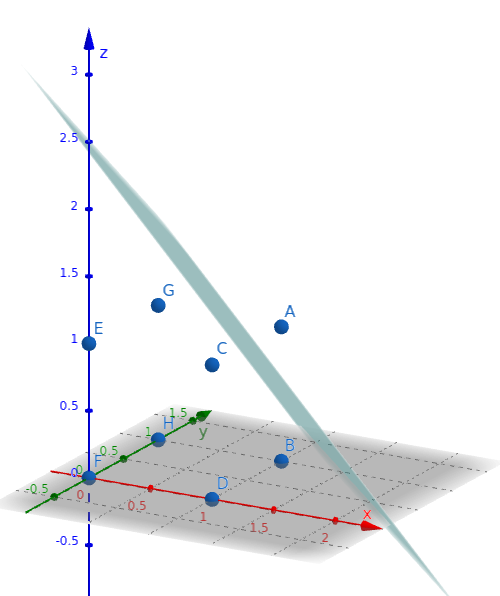
\includegraphics[width=0.4\textwidth]{cube.png}
	\caption{$f$ mapping and separating $(1,1,1)$ only}
	\label{fig:cube-png}
\end{figure}
\noindent We know that $(1,1,1)$ is the only combination for which the sum is $3$, with all other sums being $\le  2$. Using this information, we can simply modify such that when we use the step function that all results $\le 2$ give $H(z_{\neg(1,1,1)}) = 0$ and $H(z_{(1,1,1)})=1$ one by adding $-3$. That is, we know that $b=-3$ if we consider $\forall w_i = 1$, $i \in \{1,2,3\}$ intuitvely. Therefore, the perceptron diagram for function $f$ can be depicted as such:
\begin{figure}[H]
	\centering
	\begin{tikzpicture}
		\node[draw, shape=circle, scale=3] (r) at (0,0) {};
		\node[text] at (-0.2,0) {$\Sigma$ };
		\node[text] (x1) at (-3, 0) {$x_2$};
		\node[text] (f) at (3,0) {$f$ };
		\node[text] (x2) at (-3,1.5) { $x_1$ };
		\node[text] (x3) at (-3,-1.5) {$x_3$ };
		\draw[->]  (x1) to node[above,sloped] {$w_2=1$} (r);
		\draw[->]  (x2) to node[above,sloped] {$w_1=1$} (r);
		\draw[->]  (x3) to node[above,sloped] {$w_3=1$} (r);
		\path [->] (r) edge (f);
		\draw[->]  (0,-1.5) to node[right] {$b=-3$} (r);
		\draw[-] (0,-0.5) -- (0,0.5);
		\draw[-] (0.1,-0.1) -- (0.2,-0.1);
		\draw[-] (0.2,-0.1) -- (0.2,0.1);
		\draw[-] (0.2,0.1) -- (0.3,0.1);
	\end{tikzpicture}
	\caption{Rojas diagram of $f$}
	\label{fig:rojas}
\end{figure}
\newpage
\section{Question 2}
\subsection{(a)}
For hidden layer $h_1$, we find the input is
\begin{align*}
	1 \cdot -4 + -2 \cdot -2 - 1 = -1
\end{align*}
Similarly, for $h_2$ and $h_3$ respectively it is
\begin{align*}
	1 \cdot 1 + -2 \cdot 1 + 0 &= -1 \\
	1 \cdot 0 + -2 \cdot 1 + 2 &= 0
\end{align*}
Therefore, we find that the output of the hidden layer is, for each hidden layer,
\begin{align*}
	\text{tanh}_1(-1) &= -0.76159415595\ldots\\
	\text{tanh}_2(-1) &= -0.76159415595\ldots \\
	\text{tanh}_3(0) &= 0
\end{align*}
The input to the output layer, is then
\begin{align*}
	-0.76159415595 \cdot 2 + -0.76159415595 \cdot -1 + 0 \cdot 1 + 2 = 1.23840584405
\end{align*}
Therefore, the output $\hat{y}$ is then found to be
\begin{align*}
	\sigma(1.23840584405) = 0.7753 \text{              }& \text{ 4d.p.}
\end{align*}
\subsection{(b)}
We list all the related equations as such:
\begin{align*}
	z_1 &= w_1x_1 + w_4x_2 + b_1 \\
	h_1 &= \text{tanh}(z_1) \\
	z_y &= h_1w_7 + h_2w_8 + h_3w_9\\
	\hat{y} &= \sigma(z_y) \\
	L &= \frac{1}{2}\left( y-\hat{y} \right) ^2
\end{align*}
Therefore for the partial derivatives we obtain
\begin{align*}
	z_{1}_{w_1} &= x_1 \\
	h_{1}_{z_1} &= 1-h_1^2 \\
	z_{y}_{h_1} &= w_7 \\
	\hat{y}_{z_{y}} &= \hat{y}\left( 1-\hat{y} \right) \\
	L_{\hat{y}} &= \hat{y} - y
\end{align*}
We now multiply all of these values that create a single path as such:
\begin{align*}
	x_1 \cdot (1-h_1^2) \cdot w_7 \cdot \hat{y}(1-\hat{y}) \cdot (\hat{y} -y)
\end{align*}
Which after substitution obtains us
\begin{align*}
	g = 1 \cdot (1-(-0.76159415595)^2)\cdot 2 \cdot 0.77528640646(1-0.77528640464)\cdot(0.77528640646-0.7)
\end{align*}
For which the above computes to
\begin{align*}
	g= 0.01 \; \text{ 2d.p.}
\end{align*}
\newpage
\section{Question 3}
\subsection{(a)}
Two disadvantages to the sigmoid function in training neural networks:
\begin{enumerate}
	\item Vanishing gradient - large or small inputs have very little change in prediction. This can result in the network refusing to learn further.
	\item Computationally expensive - the present of exponential function means that the sigmoid function is computationally heavy.
\end{enumerate}

\noindent We first show that the sigmoid function $\sigma(x)$ has a property of being strictly increasing and non-negative. We first prove that it is strictly non-negative:
\begin{proof}
	We have that, $\forall x$ the function $e^{-x} > 0$. Using this information, we can deduce that the function $\sigma(x)$
	 \begin{align*}
		\sigma(x) = \frac{1}{1+e^{-x}}
	\end{align*}
	Is also strictly non-negative.
\end{proof}
\noindent We now show it is strictly increasing.
\begin{proof}
	That is, by differentiating, we find
\begin{align*}
	\sigma '(x) = \frac{e^{x}}{\left( e^{x}+1 \right) ^2}
\end{align*}
We know that $\forall x, e^x > 0$, therefore, we can deduce that $\forall x, \sigma'(x) >0$. We have shown that it is strictly increasing, a property which will be useful in a later proof.
\end{proof}
\noindent For a function $f(x)$ to be a probability density function, the requirement is that
\begin{align*}
	\int_{-\infty}^{+\infty} f(x) \; \mathrm{d}x = 1
\end{align*}
Otherwise, we can actually split the integral such that
\begin{align*}
	\int_{-\infty}^{+\infty} f(x) \mathrm{d} x =	\int_{-\infty} ^{1} f(x) \mathrm{d}x + \int_1^{5} f(x) \mathrm{d}x + \int_5^{+\infty} f(x) \mathrm{d}x
\end{align*}
We now calculate
\begin{align*}
	\int_1^{5} \sigma(x) \mathrm{d}x = \left[\ln\left( e^{-x}+1 \right)  \right]_{1}^{5} = 3.693\ldots
\end{align*}
However, we know that the function is strictly increasing and non-negative. Therefore, we can deduce that
\begin{align*}
	\int_{-\infty}^{1} \sigma(x) \mathrm{d}x > 0 \\
	\int_5^{+\infty} \sigma(x) \mathrm{d} x > 0 
\end{align*}
Therefore, the sum of the three integrals, denote it $y$, achieves us
\begin{align*}
	y >3.693\ldots
\end{align*}
which proves that it is not a probability density function.

\end{document}
